\appendix
\renewcommand{\theequation}{\Alph{section}.\arabic{subsection}.\arabic{equation}}
\setcounter{equation}{0}

\section{物理数学}

\subsection{線形代数}

\subsubsection{完全反対称tensorとvectorの外積、ベクトル解析の公式}

$n$階の完全反対称tensor(completely antisymmetric tensor、
\footnote{反対称(anti-symmetric)と
歪対称(skew-symmetric)は同じ意味。}
Levi-Civita symbol、
エディントンのepsilonと呼ばれる事もあるが
Edington's epsilonと洋書に書いてあることは少ない)を
\begin{align}
    \epsilon_{i_1,\dots,i_n} =
    \begin{cases}
        + 1
        &\text{
            $(i_1,\dots,t_n)$が
            $(1,\dots,n)$の偶置換
        }
    \\
        - 1
        &\text{
            $(i_1,\dots,t_n)$が
            $(1,\dots,n)$の奇置換
        }
    \\
        0
        &\text{
            else
        }
    \end{cases}
\label{completely antisymmetric tensor}
\end{align}
で定義する。
特に$(i_1,\dots,t_n)$が$(1,\dots,n)$の置換$\sigma$であるとき、
明らかにこれは置換の符号
$\mathrm{sign}(\sigma)$に一致する。

縮約されている添え字は
和を取るためだけに使っているダミーの添え字
($\sum_i a_i = \sum_j a_j$のように、
文字を変えても式の意味は変わらない)
であることに気を付けると
\begin{align}
    \epsilon_{ijk}
    \partial_i \partial_j
    &=
    \epsilon_{jik}
    \partial_j \partial_i
    =
    - \epsilon_{ijk}
    \partial_i \partial_j
\notag\\\therefore
    \epsilon_{ijk}
    \partial_i \partial_j
    &=
    0
\end{align}
のように$\epsilon$と対称tensorを潰すと必ず$0$になることが分かる。
より一般に、$\epsilon$に限らない反対称tensorと
対称tensorとの足を$2$つ以上縮約すると
必ず$0$になることも明らかだろう。

$3$階の完全反対称tensorについては公式
\begin{align}
    \epsilon_{ijk}\epsilon_{ilm}
    =
    \delta_{jl}\delta_{km}
    -
    \delta_{jm}\delta_{kl}
\label{3rd order epsilon to delta2 formula}
\end{align}
が成り立つ。
$3$次元直交座標系でvectorを成分表示すると、
外積は
\begin{align}
    (\bm{a} \times \bm{b})_i
    =
    \epsilon_{ijk}
    a_j b_k
\label{cross product}
\end{align}
と書け、$\epsilon$の反対称性から
ベクトル解析の公式
\begin{subequations}
\begin{align}
    \bm{a} \cdot (\bm{b} \times \bm{c})
    &=
    \bm{b} \cdot (\bm{c} \times \bm{a})
    =
    \bm{c} \cdot (\bm{a} \times \bm{b})
\\
    \bm{a} \times (\bm{b} \times \bm{c})
    &=
    \bm{b} (\bm{a} \cdot \bm{c})
    -
    (\bm{a} \cdot \bm{b}) \bm{c}
\\
    \nabla \times (\nabla \times \bm{c})
    &=
    \mathrm{rot}(\mathrm{rot}\ \bm{c})
    =
    \mathrm{grad}(\mathrm{div}\ \bm{c})
    -
    \Delta\ \bm{c}
    =
    \nabla (\nabla \cdot \bm{c})
    -
    (\nabla \cdot \nabla) \bm{c}
\\
    \nabla \times (\nabla \phi)
    &=
    \mathrm{rot}(\mathrm{grad}\ \phi)
    = 0
\\
    \nabla \cdot (\nabla \times \bm{A})
    &=
    \mathrm{div}(\mathrm{rot}\bm{A})
    = 0
\end{align}
\end{subequations}
は簡単に示せる。

\subsubsection{外積とAxial Vector}

実は(\ref{cross product})は外積の性質ではなく、
その定義である。
ここで使われている$\epsilon_{ijk}$は
非相対論的な$3$次元空間$\mathbb{R}$の回転群$SO(3)$の不変tensorであり、
得られた外積はvecctorのように見えるが
実は空間反転の下で負号を出すという意味で真のvectorではない。

順を追って説明していこう。
vector spaceに何らかの群$G$が作用しているとする。

\subsubsection{行列式、余因子行列と逆行列}

$D$次元正方行列$g_{\mu\nu}$の行列式(determinant)は、
抽象的には
$g_{\mu\nu}$を分解して出来る$D$個のvector
\footnote{
    うるさいことを言うと
    vectorを太字にする流儀では
    行列は太字の大文字で書くのが普通であるが、
    物理では大文字小文字の使い分けにも意味がある場合が多いので、
    行列(というか$2$階のtensor)は必ずしも大文字にも太字にもしない。
}
\begin{align*}
    \bm{a}_1 :=
    \begin{pmatrix}
        g_{11}
    \\
        g_{21}
    \\
        \vdots
    \\
        g_{D1}
    \end{pmatrix}
    ,
    \dots,
    \bm{a}_D :=
    \begin{pmatrix}
        g_{1D}
    \\
        g_{2D}
    \\
        \vdots
    \\
        g_{DD}
    \end{pmatrix}
\end{align*}
の関数
\begin{align}
    \det(g_{\mu\nu})
    :=
    \det(\bm{a}_1,\dots,\bm{a}_D)
\end{align}
であって、
以下の3つの性質を満たすもの:
\begin{subequations}
\begin{enumerate}
\renewcommand{\labelenumi}{(\roman{enumi})}
    \item 反対称性:
    \\
    どの$2$つのvectorの入れ替えのもとでも反対称
    \begin{align}
        \det(\bm{a}_1,\dots,\bm{a}_i,\dots,\bm{a}_j\dots,\bm{a}_D)
        =
        -
        \det(\bm{a}_1,\dots,\bm{a}_j,\dots,\bm{a}_i\dots,\bm{a}_D)
    \end{align}
    \item 多重線形性:
    \\
    どのvectorについても線形
    \begin{align}
        \det(\bm{a}_1,\dots,c\bm{a}_i+d\bm{b}_i\dots,\bm{a}_D)
        =
        c
        \det(\bm{a}_1,\dots,\bm{a}_i\dots,\bm{a}_D)
        +
        d
        \det(\bm{a}_1,\dots,\bm{b}_i\dots,\bm{a}_D)
    \end{align}
    \item 規格化条件:
    \\
    単位行列$\mathbbm{1}$に対して$1$を与える
    \begin{align}
        \det(\mathbbm{1}) = 1
    \end{align}
\end{enumerate}
\end{subequations}
と定義される。

等価であるが、より具体的には
行列の成分を完全反対称テンソルで潰したもの
\begin{align}
    \det(g_{\mu\nu})
    :=
    \sum_{i_1,\dots,i_D}
    \epsilon_{i_1,\dots,i_D}
    g_{1, i_1}
    \cdots
    g_{D, i_D}
\end{align}
とも定義され、$\det(g) = |g|$とも書く。
$g$の逆行列$g^{-1}$の$(\mu,\nu)$成分を
$g^{\mu\nu}$と書くことにすると
\begin{align}
    \dfrac{\partial \det(g)}{\partial g_{\mu\nu}}
    =
    g^{\mu\nu}
\end{align}
が成り立つ。

行列$g_{\mu\nu}$の$i$行と$j$列を除いたものの行列式の$(-1)^{i+j}$倍
\begin{align}
    \Delta(i,j) :=
    (-1)^{i+j}
    \begin{vmatrix}
        g_{1,1} & \dots & g_{1,j-1} & g_{1,j+1} & \dots & g_{1,D}
    \\
        \vdots & \ddots & \vdots & \vdots & \ddots & \vdots
    \\
        g_{i-1,1} & \dots & g_{i-1,j-1} & g_{i-1,j+1} & \dots & g_{i-1,D}
    \\
        g_{i+1,1} & \dots & g_{i+1,j-1} & g_{i+1,j+1} & \dots & g_{i+1,D}
    \\
        \vdots & \ddots & \vdots & \vdots & \ddots & \vdots
    \\
        g_{D,1} & \dots & g_{D,j-1} & g_{D,j+1} & \dots & g_{D,D}
    \end{vmatrix}
\end{align}
を余因子(cofactor)と呼ぶ。
余因子行列(cofactor matrix)はその$(i,j)$成分が$(j,i)$余因子で与えられるような行列$\Delta$
\begin{align}
    (\Delta)_{i,j} := \det(\Delta(j,i))
\end{align}
と定義され、
$g_{\mu\nu}$の逆行列はCramer's rule
\begin{align}
    (g^{-1})_{i,j}
    = ( g^{i,j} = )
    \dfrac{ (\Delta)_{i,j} }
    { \det(g_{\mu\nu}) }
\end{align}
で書ける事が知られている。

\subsubsection{$L^p$-norm}

$\mathbb{R}^n$または
$\mathbb{C}^n$上の
$n$次元vector $v$に対し、
実数$1\le p < \infty$の範囲で
$L^p$-normを
\begin{align}
    ||v||_p
:=
    \left(
        \sum_{i=1}^n
        |v_i|^p
    \right)^{ \dfrac{1}{p} }
\end{align}
と定義する。
$p\to\infty$の極限を
$L^\infty$-normないし最大値normと言い、
\begin{align}
    ||v||_\infty
=
    \max_i
    |v_i|
\end{align}
に一致する。
特に$n \to \infty$(つまり無限数列)の場合、
上の$p$-normを有限にするようなvectorの集合を$l^p$と呼ぶ。

測度空間についても
和を積分に置き換えることにより同様のnormが定義でき、
これを有限にする可測関数の集合を
$L^p$空間(エルピー空間、あるいはLebesgue space)
と呼ぶ。

\subsection{複素関数論}

\subsubsection{Taylor series expansion(テイラー級数展開)}

実関数$f(x)$が点$a$で無限回微分可能であるとする。
\begin{subequations}
\begin{align}
    f(x)
    &=
    \sum_{n=0}^{\infty}
    \dfrac{ f^{n}(a) }{n!}
    (x-a)^n
\label{Taylor series expansion}
\\
    f^{n}(a)
    &:=
    \dfrac{d^nf}{dx^n}\bigg|_{x=a}
\end{align}
\end{subequations}
を$f(x)$の$a$周りでのTaylor展開という。
特に
$a=0$とした場合のTaylor展開を
Maclaurin series expansion(マクローリン展開)とも言う。
Taylor展開が収束し、
かつ元の関数$f(x)$に一致するとき
$f(x)$はTaylor展開可能であるという。
例えば$\exp(-1/x^2)$は$x=0$で無限回微分可能であり
そのTaylor展開も収束するが、
恒等的に$0$になって$\exp(-1/x^2)$に一致しない。
従って$\exp(-1/x^2)$は$x=0$まわりでTaylor展開可能ではない
(このことは、$\exp(-1/x^2)$を複素関数と見たとき
$x=0$が真性特異点となっている事実を反映している)。

複素関数$f(z)$が領域$D$で正則であるとする。
点$a$を中心とする領域$D$内の任意の円$C$に対し、
$f(z)$は$C$の内部で
\begin{subequations}
\begin{align}
    f(z)
    &=
    \sum_{n=0}^{\infty}
    \dfrac{f^{(n)}(a)}{n!}
    (z-a)^n
\\
    f^{(n)}(a)
    &=
    \dfrac{n!}{2 \pi i}
    \oint_C dz_0\dfrac{f(z_0)}{(z_0 - a)^{n+1}}
\label{Cauchy's integral formula}
\end{align}
\end{subequations}
とべき級数展開できる。
なお
(\ref{Cauchy's integral formula})
は$f(a)$の$n$階の導関数を与え、
特に$n=0$の場合を指して
Cauchy's integral formula(コーシーの積分公式)
と呼ぶことがある。

Taylor展開可能な実関数または複素関数を解析関数(analytic function)という。
$f(z)$が複素関数の意味で$z$により微分できるとき
正則関数(holomorphic function)と言うのであったが、
複素関数は領域$D$で正則であれば無限階微分可能であり、
しかもその導関数も$D$で正則なので、
複素関数に対して解析関数と正則関数はほとんど区別しない。

\subsubsection{Laurent series expansion(ローラン級数展開)}

\begin{wrapfigure}[7]{r}[5pt]{107pt}
  \centering
  

\tikzset{every picture/.style={line width=0.75pt}} %set default line width to 0.75pt        

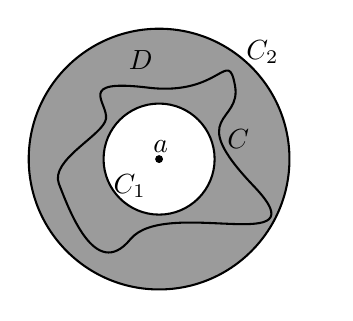
\begin{tikzpicture}[x=0.4,y=0.4,yscale=-1,xscale=1]
%uncomment if require:
\path (0,240.79999542236328);
%set diagram left start at 0, and has height of 240.79999542236328

%Shape: Circle [id:dp6258198346024846] 
\draw  [fill={rgb, 255:red, 155; green, 155; blue, 155 }  ,fill opacity=1 ] (0.77,120.35) .. controls (0.77,55.3) and (53.5,2.57) .. (118.55,2.57) .. controls (183.6,2.57) and (236.32,55.3) .. (236.32,120.35) .. controls (236.32,185.4) and (183.6,238.12) .. (118.55,238.12) .. controls (53.5,238.12) and (0.77,185.4) .. (0.77,120.35) -- cycle ;
%Shape: Circle [id:dp07560041299187703] 
\draw  [fill={rgb, 255:red, 255; green, 255; blue, 255 }  ,fill opacity=1 ] (68.39,120.35) .. controls (68.39,92.65) and (90.85,70.19) .. (118.55,70.19) .. controls (146.25,70.19) and (168.71,92.65) .. (168.71,120.35) .. controls (168.71,148.05) and (146.25,170.51) .. (118.55,170.51) .. controls (90.85,170.51) and (68.39,148.05) .. (68.39,120.35) -- cycle ;
%Shape: Circle [id:dp4185264747557642] 
\draw  [fill={rgb, 255:red, 0; green, 0; blue, 0 }  ,fill opacity=1 ] (116,120.35) .. controls (116,118.94) and (117.14,117.8) .. (118.55,117.8) .. controls (119.96,117.8) and (121.1,118.94) .. (121.1,120.35) .. controls (121.1,121.76) and (119.96,122.9) .. (118.55,122.9) .. controls (117.14,122.9) and (116,121.76) .. (116,120.35) -- cycle ;
%Shape: Polygon Curved [id:ds19792072871438626] 
\draw   (108.6,55.8) .. controls (174.6,63.8) and (180.6,18.8) .. (187.1,53.8) .. controls (193.6,88.8) and (141,78.8) .. (204.1,144.8) .. controls (267.2,210.8) and (124.6,153.8) .. (92.6,192.8) .. controls (60.6,231.8) and (36.72,164.55) .. (28.1,142.8) .. controls (19.47,121.05) and (68.77,98.46) .. (70.6,83.8) .. controls (72.43,69.14) and (42.6,47.8) .. (108.6,55.8) -- cycle ;

% Text Node
\draw (120,108.8) node    {$a$};
% Text Node
\draw (102,30.8) node    {$D$};
% Text Node
\draw (92,144.8) node    {$C_{1}$};
% Text Node
\draw (212,23.8) node    {$C_{2}$};
% Text Node
\draw (190,101.8) node    {$C$};

\end{tikzpicture}

  \caption{単純閉曲線$C$}
\end{wrapfigure}
複素関数$f(z)$が点$a$を孤立特異点に持つとする。
また、点$a$を中心とする円$C_1, C_2$
($C_1$の中に$a$以外の特異点があっても良く、
$C_2$は$C_1$の外側にあるとする)
によって囲まれる領域を$D$とする。
$C_1, C_2$上、領域$D$のいずれにも特異点がないとき、
領域$D$内の任意の$z$に対し、
$D$内にあって$C_1$を囲むような単純閉曲線$C$を使って
\begin{subequations}
\begin{align}
    f(z)
    &= \sum_{n=-\infty}^{\infty}
        c_n (z-a)^n
\label{Laurent series expansion}
\\
    c_n
    &:= \dfrac{1}{2 \pi i}
    \oint_C dz_0 \dfrac{f(z_0)}{(z_0 - a)^{n+1}}
\end{align}
\end{subequations}
が成り立つ。
これを$f(z)$の$a$周りでのLaurent級数展開という。
特に(\ref{Laurent series expansion})の右辺のうち
$c_{-n}\ (n > 0)$が現れる項を特異部(singular part、主要部、principal part)、
$c_{n}\ (n \ge 0)$が現れる項を正則部(regular part、analytic part)という。

\subsubsection{極(pole)、真性特異点(essential singularity)、零点(zero)}

極とは、以下に定める孤立特異点の一種である。
$f(z)$が$a$を$m\ (>0)$位の極($m$-th order pole)
に持つとは、
$f(z)$のLaurent級数展開が$c_{-m} \neq 0$かつ
$n>m$に対し$c_{-n}=0$を満たすことを言う。
特に$1$位の極を単純極(simple pole)、
$2$位の極を二重極(double pole)、
$3$位ならtriple pole、などともいう。

Laurent展開の特異部が有限次で切れず
負べきの項が無限個現れる場合、
$a$を真性特異点(essential singularity)という。

$f(z)$が$a$を$m$位の零点($m$-th order zero)
に持つとは、
$f(z)$のTaylor級数展開
(\ref{Taylor series expansion})
が$c_{m} \neq 0$かつ
$0 \le n < m$に対し$c_{n}=0$を満たすことを言う。
正則関数の零点は孤立し、
この事実を零点孤立の原理という。

\subsubsection{留数定理(Residue theorem)}

Laurent級数展開
\begin{align}
    f(z)
    &= \sum_{n=-\infty}^{\infty}
        c_n (z-a)^n
\end{align}
において、
$\Res{f(z)dz, a} := c_{-1}$を
$f(z)$の点$z=a$における留数(Residue)という。
ただし本来これはRiemann球面$\mathbb{C}P^1$上の
微分形式に対し定義されるものだと示すため、
単に$f(z)$ではなく$f(z)dz$と書いた。
特に、
$f(z)$が$a$を$m$位の極
に持つときは
\begin{align}
    \Res{f(z)dz, a}
    =
    \lim_{z \to a}
    \dfrac{1}{(m-1)!}
    \dfrac{d^{m-1}}{dz^{m-1}}
    \bigg[
        (z-a)^m f(z)
    \bigg]
\end{align}
が成り立つ。
$f(z)$が単純閉曲線$C$内で
$n$個の孤立特異点$a_1,\dots,a_n$を除き正則であるとき
\begin{align}
    \oint_C dz\ f(z)
    =
    2 \pi i \sum_{k=1}^n
    \Res{f(z)dz, a_k}
\end{align}
が成り立つ。

\subsubsection{Morera's theorem(モレラの定理)}

以下の意味で、Cauchyの積分定理の逆が成り立つ:
単連結領域$D$で$f(z)$が連続で、
\begin{align}
    \oint_C dz\ f(z) = 0
\end{align}
が$D$内の任意の閉曲線$C$に対し成り立つとする。
このとき$f(z)$は$D$上で正則である。

\subsection{特殊関数}

\subsubsection{指数関数}

指数関数(exponential function)を
\begin{align}
    \exp(x)
    :=
    \sum_{n=0}^\infty
    \dfrac{x^n}{n!}
\end{align}
により定める。
この級数は複素平面全体で絶対収束するため、
$\exp(z)$は整関数
(entire function、複素平面全体で正則な関数)を与える。

\subsubsection{三角関数、双曲線関数}

余弦(cosine)関数、
正弦(sine)関数、
正接(tangent)関数を
指数関数を用いて
\begin{align}
    \cos\theta &:= \dfrac{e^{i\theta} + e^{-i\theta}}{2}
\\
    \sin\theta &:= \dfrac{e^{i\theta} - e^{-i\theta}}{2i}
\\
    \tan\theta &:= \dfrac{\sin\theta}{\cos\theta}
\end{align}
と定義する。
これらを総称して三角関数
(trigonometric function、circular function)
という。

同様に双曲線関数(hyperbolic function)を
\begin{align}
    \cosh\theta
    &:=
    \dfrac{e^{\theta} + e^{-\theta}}{2}
    =
    \cos(-i\theta)
\\
    \sinh\theta
    &:=
    \dfrac{e^{\theta} - e^{-\theta}}{2}
    =
    i\sin(-i\theta)
\\
    \tanh\theta
    &:=
    \dfrac{\sinh\theta}{\cosh\theta}
\end{align}
と定義する。
それぞれ
hyperbolic cosine、
hyperbolic sine、
hyperbolic tangentと言うが、
$\cosh, \sinh, \tanh$の記号は
cosine hyperbolic(またはコッシュ)、
sine hyperbolic(またはシンチ)、
tangent hyperbolic(またはタンチ)
などと発音される。
native English speakerでも
シンチとかタンチとか言う人は居るが、
分かりづらいだけでなく
はっきり言ってクソダサいので
cosine hyperbolic、sine hyperbolic
などという方が良いと思う。

\subsubsection{$\Gamma$関数}

$\Gamma$関数は$\Re z > 0$の複素数$z$に対し
\begin{align}
    \Gamma(z)
    := \int_0^\infty dt\ t^{z-1} e^{-t}
\end{align}
により定義され、
その性質
$\Gamma(1) = 1, \Gamma(z+1) = z\Gamma(z)$
から階乗(factorial)
\begin{align}
    \Gamma(n+1) &= n!
    \quad
    (n \in \mathbb{N}_{\ge0})
\end{align}
の複素数への一般化を与える。

重要な応用として、
Gaussian integral(ガウス積分)
\begin{align}
    I :=
    \Gamma\left(\dfrac{1}{2}\right)
    =
    \int_{0}^{\infty} dt\ t^{-1/2}e^{-t}
    =
    2
    \int_{0}^{\infty} dx\ e^{-x^2}
    =
    \int_{-\infty}^{\infty} dx\ e^{-x^2}
    > 0
    \quad(t=x^2)
\end{align}
を求める事を考えよう。
極座標に書き換えると
\begin{align}
    I^2 &=
    \int_{-\infty}^{\infty} dx
    \int_{-\infty}^{\infty} dy
    \ 
        e^{-(x^2 + y^2)}
=
    \int_0^{\infty} dr
    \int_0^{2\pi} r d\theta
    \ 
        e^{-r^2}
\notag\\&=
    2 \pi
    \int_0^{\infty} dr
    \ r 
        e^{-r^2}
=
    \pi
    \int_0^{\infty} dt\ e^{-t}
    \quad(t:=r^2,\ dt = 2 r dr)
\notag\\&=
    \pi\Gamma(1)
    = \pi
\end{align}
すなわち
$\Gamma\left(\dfrac{1}{2}\right)
= I = \sqrt{\pi}$
が求まる。
初等的な置換積分により
\begin{align}
    \int_{-\infty}^{\infty} dx\ e^{-ax^2}
    =
    \sqrt{
        \dfrac{\pi}{a}
    }
\end{align}
もすぐ分かり、より一般に
$n \in \mathbb{N}_{\ge0}$に対して
\begin{align}
    \Gamma\left( n + \dfrac{1}{2} \right)
    &=
    \int_0^\infty dt\ t^{n-1/2} e^{-t}
\notag\\&=
    \left[
        \left(
            -
            \dfrac{d}{da}
        \right)^n
        \int_0^\infty dt\ t^{-1/2} e^{-at}
    \right]_{a=1}
\notag\\&=
    \left[
    \left(
        -
        \dfrac{d}{da}
    \right)^n
        a^{-1/2}
        \int_0^\infty a dt\ (at)^{-1/2} e^{-at}
    \right]_{a=1}
\notag\\&=
    \left[
    \left(
        -
        \dfrac{d}{da}
    \right)^n
    \sqrt{
        \dfrac{\pi}{a}
    }
    \right]_{a=1}
\notag\\&=
    \dfrac{(2n-1)!!}{2^{n}}\sqrt{\pi}
\end{align}
が得られる。
ただしdouble factorial(二重階乗)を
偶数、奇数それぞれについて
\begin{subequations}
\begin{align}
    (2n)!!
    &:=
    \prod_{i=1}^n (2i)
    =2\cdot4\cdot6\cdots(2n-2)(2n)
\\
    (2n-1)!!
    &:=
    \prod_{i=1}^n (2i-1)
    =
    1\cdot3\cdot5\cdots(2n-3)(2n-1)
\end{align}
\end{subequations}
と定義した。

$\Gamma$関数の$\Re z < 0$への解析接続は
Euler's reflection formula
\begin{align}
    \Gamma(z) \Gamma(1-z)
    =
    \dfrac{\pi}{\sin(\pi z)}
\label{Euler's reflection formula}
\end{align}
で与えられ、
この公式からも
$\Gamma \left(\dfrac{1}{2}\right) = \sqrt{\pi}$
が確かめられる。
$\Gamma$関数は零点を持たないが
(\ref{Euler's reflection formula})からも分かるように
$n \in \mathbb{N}_{\ge0}$に対して
$x = - n$を$1$位の極に持ち、
その周りで
\begin{align}
    \Gamma(x)
    &=
    \dfrac{(-1)^n}{n!}
    \left(
        \dfrac{1}{x+n} - \gamma
        + \sum_{k=1}^n \dfrac{1}{k}
    \right)
    + \mathcal{O}(x+n)
\\
    \gamma
    &:=
    \lim_{n\to\infty}
    \left(
        \sum_{k=1}^n \dfrac{1}{k} 
        -
        \log n
    \right)
    \simeq 0.5772
\end{align}
と展開できる。
ただし$\gamma$は
Euler-Mascheroni constant(オイラー定数)である。


\subsection{Fourier変換、Fourier級数展開}

\subsubsection{Fourier級数展開}

周期$2L$の周期関数$f(x)$、
あるいは区間$(a, a + 2L)$を定義域とする関数$f(x)$を
周期関数に拡張したものについて
\begin{subequations}
\begin{align}
    \tilde{f}(x)
    &:=
    \sum_{n=-\infty}^\infty
    c_n e^{ i\frac{n \pi}{L}x }
\\
    c_n
    &:=
    \dfrac{1}{2L} \int_{-L}^L dx\ 
    f(x) e^{ - i\frac{n \pi}{L}x }
\end{align}
\end{subequations}
を複素Fourier series(フーリエ級数)、
\begin{subequations}
\begin{align}
    \tilde{f}(x)
    &:=
    \dfrac{a_0}{2}
    +
    \sum_{n=1}^\infty
    \left(
        a_n \cos \dfrac{n \pi}{L}x
        +
        b_n \cos \dfrac{n \pi}{L}x
    \right)
\\
    a_n
    &:=
    \dfrac{1}{L} \int_{-L}^L dx\ 
    f(x) \cos\dfrac{n \pi}{L}x
\\
    b_n
    &:=
    \dfrac{1}{L} \int_{-L}^L dx\ 
    f(x) \sin\dfrac{n \pi}{L}x
\end{align}
\end{subequations}
をFourier seriesなどという。
特に$\forall n$に対して
$a_n = 0$のときFourier正弦展開、
$b_n = 0$のときFourier余弦展開
などということもある。

$f(x)$が区分的になめらか、
つまり$f(x), f'(x)$がともに区分的に連続ならば
そのFourier級数は各点収束し、収束先は
\begin{align}
    \tilde{f}(x) = \dfrac{f(x+0) + f(x-0)}{2}
\end{align}
で与えられる。
$f(x)$が連続ならさらに強くFourier級数は関数列として一様収束するが、
不連続関数のFourier級数は一様収束せず、
広義一様収束、ないしコンパクト一様収束
(uniformly convergent on compact sets)
しかしない。
不連続点$x = a$ s.t.
$\mathrm{Disc}(f,a) := f(a+0) - f(a-0) \neq 0$の付近では
振幅$\mathrm{Disc}(f,a) \times 0.08949\dots$程度の振動が起こり、
ギブス現象(Gibbs phenomenon)とか呼ばれる。
激しく振動する成分はRiemann-Lebesgue lemmaより積分に寄与しないので、
$L^2$-normで見る限り(\ref{convergence of norm})と全く同様に
\begin{subequations}
\begin{align}
    \lim_{N\to\infty}\bigg|\bigg|
        f(x) - \tilde{f}_N(x)
    \bigg|\bigg|^2
    &=
    \lim_{N\to\infty}\int dx
    \Big| f(x) - \tilde{f}_N(x) \Big|^2
    = 0
\\
    \tilde{f}_N(x)
    &:=
    \sum_{n=-N}^N
    c_n e^{ i\frac{n \pi}{L}x }
\end{align}
\end{subequations}
のように収束している、ということである。

\subsubsection{Fourier変換}

周期関数でないより一般の関数もFourier級数と同様に
三角関数で展開したいというのは自然な要求だろう。
特にこれは微分方程式を解くために役立つ。
急減少関数$f(x)$のFourier transform(フーリエ変換)$\tilde{f}(k)$
および
inverse Fourier transform(逆フーリエ変換)を
\begin{subequations}
\begin{align}
    \tilde{f}(k)
    &:=
    \int dx\ f(x) e^{-ikx}
\\
    f(x)
    &=
    \dfrac{1}{2\pi}\int dk\ 
    \tilde{f}(k) e^{+ikx}
\end{align}
\end{subequations}
で定める。
$\dfrac{1}{2\pi}$を
Fourier変換(逆変換でなく)の定義に付けて
$\tilde{f}(k)=\dfrac{1}{2\pi}\int dx\ f(x) e^{-ikx}$
としたり、
$k$の符号を逆にして
$\tilde{f}(k)=\int dx\ f(x) e^{+ikx}$としたり、
波動関数の規格化を気にする量子力学では
$\dfrac{1}{\sqrt{2\pi}}\int dk\ \tilde{f}(k) e^{+ikx}$
のように$\dfrac{1}{\sqrt{2\pi}}$が変換と逆変換の両方に現れたり、
数値計算や結晶学では角周波数でなく周波数を用いて
$\tilde{f}(k)=\int dx\ f(x) e^{+2\pi ikx}$としたり、
とにかく無数の流儀があるが、本質積な違いは何もない。

上の逆変換はDirac delta関数のFourier表示
\begin{align}
    \delta(x-y) = \dfrac{1}{2\pi}\int dk\ e^{ik(x-y)}
\end{align}
により正当化される。

Fourier変換は不確定性関係という良くない性質を持つため、
画像処理などの分野ではwavelet解析という拡張を考えることがある。

\section{量子力学の公式}

記号が煩雑になるのを避けるため、
以下では誤解の恐れがない場合は
適宜operatorを表す$\hat{}$を省略する。

\subsection{Operatorの基本的な性質}

\subsubsection{交換関係・反交換関係}

証明は読者の演習問題とする。
\begin{align}
    [\hat{A}, \hat{B}] &= - [\hat{B}, \hat{A}]
\\
    \{\hat{A}, \hat{B}\} &= \{\hat{B}, \hat{A}\}
\\
    [\hat{A}, \hat{B}\hat{C}]
   &=
   \hat{B}[\hat{A}, \hat{C}]
+
    [\hat{A}, \hat{B}] \hat{C}
\label{A,BC to B(A,C) + (A,B)C}
\\
    [\hat{A}\hat{B}, \hat{C}]
   &=
   \hat{A}\{\hat{B}, \hat{C}\}
-
    \{\hat{A}, \hat{C}\} \hat{B}
\\
    \left(\hat{A}\hat{B}\right)^\dagger
    &=
    \hat{B}^\dagger\hat{A}^\dagger
\\
    [\hat{A}, \hat{B}]^\dagger
    &=
    [\hat{B}^\dagger, \hat{A}^\dagger]
\end{align}
特に(\ref{A,BC to B(A,C) + (A,B)C})は
繰り返し使うことにより
\begin{align}
    [\hat{A}, \hat{B}_1\hat{B}_2\cdots\hat{B}_n]
   &=
   \sum_{i=1}^n
   \hat{B}_1\cdots\hat{B}_{i-1}
   [\hat{A}, \hat{B}_i]
   \hat{B}_{i+1}\cdots\hat{B}_n
\end{align}
と拡張できる。

\subsubsection{Baker-Campbell-Hausdrff formula}

Baker-Campbell-Hausdrff formulaは
\begin{align}
    e^{\hat{A}} e^{\hat{B}}
    &=
    \exp\left(
        \hat{A} + \hat{B}
        + \dfrac{1}{2}[\hat{A},\hat{B}]
        + \dfrac{1}{12}[\hat{A} - \hat{B},[\hat{A},\hat{B}]]
        + \cdots
    \right)
\label{BCH formula}
\end{align}
である。証明のためには
$e^{\hat{C}(t)}
= e^{t\hat{A}} e^{t\hat{B}}$
すなわち$\hat{C}(t) = \log (
    e^{t\hat{A}} e^{t\hat{B}}
)$とおき、
右辺のTaylor展開を計算した後
$t=1$とおけばよい
(\ref{proof for unitary transf formula for operator}
も参照のこと)。
特に交換関係が$c$-数
$[\hat{A},\hat{B}]=c$の場合は
交換子を$2$回以上取ると必ず消えるため
\begin{align}
    e^{\hat{A}} e^{\hat{A}}
    &=
    \exp\left(
        \hat{A} + \hat{B}
        + \dfrac{1}{2}c
    \right)
\label{simpler BCH formula}    
\end{align}
となる。

\subsection{Unitary Transformation}

(\ref{BCH formula})を示すのと全く同様の論法で、
Hermitianとは限らない任意のoperator $A, B$に対して
\begin{align}
    e^A B e^{-A}
    &=
    B + [A,B] + \dfrac{1}{2!}[A,[A,B]]
    +
    \dfrac{1}{3!}[A,[A,[A,B]]]
    +
    \cdots
\label{unitary transf formula for operator}
\end{align}
が示せるが、ここでは一応証明を載せておこう。

\subsubsection{Taylor展開を用いた証明}
\label{proof for unitary transf formula for operator}

記号$C_i$を漸化式
\begin{align}
    \mathrm{C}_0(A,B)
    :=
    B
,\qquad
    \mathrm{C}_{n+1}(A,B)
    :=
    [A,\mathrm{C}_{n}(A,B)]
\end{align}
で定義すると、示すべき式
(\ref{unitary transf formula for operator})は
\begin{align}
    e^{A} B e^{-A}
    &=
    \sum_{n=0}^\infty
    \dfrac{1}{n!}
    \mathrm{C}_{n}(A,B)
\label{rewrite of unitary transf of operator}
\end{align}
となる。
これを示すために実parameter $s$を導入し、
左辺を$s=0$の周りで展開する:
\begin{subequations}
\begin{align}
    e^{sA} B e^{-sA}
    &=
    e^{sA} \mathrm{C}_{0}(A,B)e^{-sA}
\\
    \dfrac{d}{ds}\bigg[
        e^{sA} B e^{-sA}
    \bigg]
    &=
    Ae^{sA} B e^{-sA}
    -
    e^{sA} B A e^{-sA}
    =
    e^{sA} [A,B]e^{-sA}
    =
    e^{sA} \mathrm{C}_{1}(A,B) e^{-sA}
\end{align}
\end{subequations}
ここで$k \ge 0$について
\begin{align}
    \dfrac{d^k}{ds^k}\bigg[
        e^{sA} B e^{-sA}
    \bigg]
    =
    e^{sA} \mathrm{C}_{k}(A,B) e^{-sA}
\end{align}
を仮定すると
\begin{align}
    \dfrac{d^{k+1}}{ds^{k+1}}
    \bigg[
        e^{sA} B e^{-sA}
    \bigg]
&=
    \dfrac{d}{ds}\bigg[
        e^{sA} \mathrm{C}_{k}(A,B) e^{-sA}
    \bigg]
\notag\\&=
    A e^{sA} \mathrm{C}_{k}(A,B) e^{-sA}
    -
    e^{sA} \mathrm{C}_{k}(A,B) Ae^{-sA}
\notag\\&=
    e^{sA} [A,\mathrm{C}_{k}(A,B)] e^{-sA}
\notag\\&=
    e^{sA}  \mathrm{C}_{k+1}(A,B) e^{-sA}
\end{align}
を得るため、帰納法から任意の$n$について
\begin{align}
    \dfrac{d^n}{ds^n}\bigg[
        e^{sA} B e^{-sA}
    \bigg]
    =
    e^{sA} \mathrm{C}_{n}(A,B) e^{-sA}
\end{align}
が示された。
これにより、左辺の$s=0$周りのTaylor級数を得る:
\begin{align}
    e^{sA} B e^{-sA}
&=
    \sum_{n=0}^\infty
        \dfrac{1}{n!}
    \bigg[
        \dfrac{d^n}{ds'^n}
        \bigg(
            e^{s'A} B e^{-s'A}
        \bigg)
    \bigg]_{s'=0}
    s^n
\notag\\&=
    \sum_{n=0}^\infty
        \dfrac{1}{n!}
    \bigg[
        \mathrm{C}_{n}(A,B)
    \bigg]
    s^n
\notag\\&=
    \sum_{n=0}^\infty
        \dfrac{s^n}{n!}
    \mathrm{C}_{n}(A,B)
\end{align}
最後に$s=1$と置けば
\footnote{
与えられた$A, B$に対し、
この級数展開の収束半径が$1$より大きいことは仮定する。
もともとoperatorの関数はTaylor展開
(\ref{function of operator})
で定義されていたので、
Taylor展開出来ない場合を考える必要はない。
}、
左辺の展開が右辺に一致したことになり、
望む公式
(\ref{rewrite of unitary transf of operator})
を得る。

\subsubsection{特殊な場合}

特に交換関係が$c$-数の場合$[\hat{A}, \hat{B}] = c$には
\begin{align}
    e^{ \hat{A} } \hat{B} e^{ - \hat{A} }
    &=
    \hat{B} + c
\label{finite translation of operator}
\end{align}
が得られ、
operatorの固有値の原点をずらす操作になっていることが分かる。
また、(\ref{unitary operator})の直下で指摘したように
Hermitian operator $\hat{O} = \hat{O}^\dagger$を使って
$\hat{A} = i \hat{O}$と取った場合は
$ e^{ \hat{A} } \hat{B} e^{ - \hat{A} } $
は$\hat{B}$のunitary transformationとなっている。

以上の2つの事実を合わせると、
例えば正準変数
$[\hat{q}_i, \hat{p}_j] = i\hbar\delta_{ij}$
について$\hat{A} = - \dfrac{a}{i\hbar} \hat{p}_j,
\hat{B} = \hat{q}_i$
として公式を使うことで
\begin{align}
    e^{ - \frac{a}{i\hbar} \hat{p}_j }
        \hat{q}_i
    e^{ \frac{a}{i\hbar} \hat{p}_i }
    &=
    \hat{q}_i + a \delta_{ij}
\end{align}
が言える。
これは運動量が並進対称性に対応する保存量であることを反映しており、
より一般の対称性変換に対応する保存量についても
類似の結果が知られている。

\subsection{保存電荷と対称性変換の生成子}

\begin{align}
    \ket{ \bm{x} + \bm{a} }
    &=
    \exp\left(
        \dfrac{ \bm{a} \cdot \hat{\bm{p}} }
        { i\hbar }
    \right)
    \ket{ \bm{x} }
\end{align}

\subsubsection{Ehrenfest Theorem}

正準変数$[\hat{q}_i, \hat{p}_j] = i\hbar\delta_{ij}$
についてはさらに興味深い事実が成り立つ。
$C_n := \dfrac{1}{i\hbar} [\hat{q}^n_i, \hat{p}_j]$について
\begin{align}
    C_{n+1}
    &=
    \dfrac{1}{i\hbar}
    [\hat{q}^{n+1}_i, \hat{p}_j]
    =
    \hat{q}_i 
    \dfrac{1}{i\hbar}
    [\hat{q}_i^n, \hat{p}_j]
    +
    \dfrac{1}{i\hbar}
    [\hat{q}_i, \hat{p}_j] \hat{q}_i^n
    =
    \hat{q}_i C_n
    +
    \delta_{ij} \hat{q}_i^n
\end{align}
なる漸化式が導けるが、
これは初期条件
$C_0  = 0, C_1 = \delta_{ij}$のもとで
容易に
\begin{align}
    C_{n+1} &= 
    \dfrac{1}{i\hbar}
    [\hat{q}^{n+1}_i, \hat{p}_j]
    = \delta_{ij} (n+1) \hat{q}^n
\label{differential by commutator}
\end{align}
と解け、多項式の微分と同じ振る舞いを与える。
全く同様に
$\dfrac{1}{i\hbar}
[\hat{q}_i, \hat{p}^{n+1}_j]
= \delta_{ij} (n+1) \hat{p}^n$
も示される。
一般にoperatorの関数$F$の定義
(\ref{function of operator})
はTaylor展開で与えられていたので、
\begin{align}
    \dfrac{1}{i\hbar}
    [F(\{ \hat{q} \},\{ \hat{p} \}), \hat{p}_i]
    &=
    \dfrac{
        \partial F(\{ \hat{q} \},\{ \hat{p} \})
    }{
        \partial q_i
    }
\\
    \dfrac{1}{i\hbar}
    [\hat{q}_j, F(\{ \hat{q} \},\{ \hat{p} \})]
    &=
    \dfrac{
        \partial F(\{ \hat{q} \},\{ \hat{p} \})
    }{
        \partial p_j
    }
\end{align}
なる公式が得られる。

任意のoperator $\hat{O}$に対し、
そのHeisenberg表示(Heisenberg描像、Heisenberg picture)を
\begin{align}
    \hat{O}(t)
    :=
    \exp\left(
        -\dfrac{\hat{H} t}{i\hbar}
    \right)
        \hat{O}
    \exp\left(
        +\dfrac{\hat{H} t}{i\hbar}
    \right)
\end{align}
のように定義する。
$\hat{H}$のSchr\"odinger描像とHeisenberg描像は
一致する。
また、もちろんSchr\"odinger描像で
$\hat{O}$自身が顕わに$t$に依存している場合も
Heisenberg描像は同様に定義できる。
Heisenberg描像のoperator
$F(\{ \hat{q} \},\{ \hat{p} \}, t)$と
$\hat{H}$との交換関係は
\begin{align}
    \dfrac{d}{d t}
    F(\{ \hat{q} \},\{ \hat{p} \}, t)
    =
    \dfrac{1}{i\hbar}
    [F(\{ \hat{q} \},\{ \hat{p} \}, t), \hat{H}]
    + \dfrac{\partial}{\partial t}
    F(\{ \hat{q} \},\{ \hat{p} \}, t)
    \label{Heisenberg e.o.m}
\end{align}
となり、Heisenberg equation of motionと呼ばれる。
これはPoisson括弧で書かれた正準方程式(\ref{Hamilton e.o.m. in Poisson bracket})
ないし任意の関数$F$の時間発展(\ref{time evolution in Poisson bracket})
と同一の構造であり、
量子化とは
$\{A, B\}_{ \mathrm{P} }$
を
$\dfrac{1}{i\hbar} [\hat{A}, \hat{B}]$
で置き換える操作である、という
Bohrの対応原理(correspondence principle)をある意味で正当化する。
もちろん\ref{subsubsec: CCR}節で述べたように、
一般にある古典力学系に対して
対応する量子力学系は一意に定まらないので
「古典系を量子化する」という操作はwell-definedではなく、
現代的にはむしろ
量子力学を十分低energyでmacroscopicな系に適用すると
古典力学を再現する、という理解が正しい。
